% Dokumentenklasse
\documentclass[a4paper,11pt,DIV=11,twoside]{scrreprt} % 

% Packages
%Datum und Uhrzeit
\usepackage{datetime}

%Encoding
\usepackage[utf8]{inputenc}
\usepackage{lmodern}

%Graphikpakete
\usepackage{graphicx}
\usepackage{xcolor}
\usepackage{tikz}
\usetikzlibrary{arrows, snakes, backgrounds}
\usepackage{wrapfig}

% Farben der THI
\definecolor{THIblue}{rgb}{0.0078,0.1176,0.4705}

\usepackage[ngerman]{babel}

%Zitierumgebung
%\usepackage{cite}% Zitieren
\usepackage[backend=biber,]{biblatex}
%\usepackage{bibgerm}% Literatur in Deutscher DIN
\usepackage[babel,german=quotes]{csquotes}
\bibliography{ref/ref_liste} % Pfad und Datei der Ref-Datenbank

%URL-Umgebung
\usepackage{url}
\renewcommand{\UrlFont}{\small\tt\color{THIblue}}

%Mathematik
\usepackage{amsmath}
\usepackage{amssymb}
\usepackage{mathtools}

%Quellcode
\usepackage{listings}
\lstset{literate=%
    {Ö}{{\"O}}1
    {Ä}{{\"A}}1
    {Ü}{{\"U}}1
    {ß}{{\ss}}1
    {ü}{{\"u}}1
    {ä}{{\"a}}1
    {ö}{{\"o}}1
    {~}{{\textasciitilde}}1
}

\definecolor{gray}{rgb}{0.5, 0.5, 0.5}
\lstset{% general command to set parameter(s)
	basicstyle=\tiny\ttfamily,%\small, % print whole listing small
	keywordstyle=\color{THIblue}\bfseries\underbar,% underlined boldblack keywords
	identifierstyle=, % nothing happens
	commentstyle=\color{green}, % white comments
	stringstyle=\color{red}\ttfamily, % typewriter type for strings
	showstringspaces=false, % no special string spaces
	%numbers=left,
	%numberstyle=\color{gray},
	%numbersep=5pt,
	captionpos=b,
	breaklines=true}
	
% Define Language
\lstdefinelanguage{log}
{
  % list of keywords
  morekeywords={
    idVendor,
    idProduct,
    bInterfaceClass,
    bInterfaceSubClass,
    bInterfaceProtocol
  },
  sensitive=false, % keywords are not case-sensitive
  %alsodigit={0482},
  morecomment=[l]{//}, % l is for line comment
  morecomment=[s]{/*}{*/}, % s is for start and end delimiter
  morestring=[b]" % defines that strings are enclosed in double quotes
}

\lstdefinelanguage{tikz}
{
  % list of keywords
  morekeywords={
	above,
	align,
  	begin,
	below,
  	caption,
	draw,
	end,
	every,
	fill,
	label,
  	line,
	minumum,
	node,
	rectangle,
	right,
	scale,
	size,
  	style,
	of,
  	width,
  	xshift,
  	yshift
  },
  sensitive=false, % keywords are not case-sensitive
  %alsodigit={0482},
  keywordstyle=\color{THIblue}\bfseries,
  morecomment=[l]{//}, % l is for line comment
  morecomment=[s]{/*}{*/}, % s is for start and end delimiter
  morestring=[b]" % defines that strings are enclosed in double quotes
}

%Microtypographie
\usepackage{microtype}

%Kopf und Fußzeilen
\usepackage{scrpage2} 	% Kopf & Fußzeile im KOMA Stil
\pagestyle{scrheadings}	% Aktiviert Verwendung vordefinierter Kolumnentitel
\clearscrheadfoot 		% alle Standard-Werte und Formatierungen löschen
\setkomafont{pagehead}{\scshape}	% Schriftart in Kopfzeile, \scshape = Kapitelchen
\automark[chapter]{section} % [linke Seite]{rechte Seite}
%\ohead{\def\pagestyle{PDTS}{\hrulefill
\includegraphics[width = 6cm]{bilder/thi_logo_quer_cropped}}}
\ohead{
\includegraphics[width = 6cm]{bilder/thi_logo_quer_cropped}}

%\ihead{\textsc{Abschlussarbeit}}
\ihead{\headmark}

%\setheadwidth[0pt]{textwithmarginpar}
\ofoot{\vspace{-0.3cm} \pagemark} 						
\ifoot{\vspace{-0.3cm} Dominik Gunther Florian Schlecht} 
				
%\setheadtopline{.4pt}				
\setheadsepline{.2pt}
\setfootsepline{.4pt}	% Trennlinie Fußzeile und Textkörper

%------------------------------------------------------------------
%% Längenanpassungen
%------------------------------------------------------------------
\setlength{\headsep}{10mm}		% Textabstand zur Kopfzeile
\setlength{\footskip}{15mm}		% Abstand zur Fußzeile
\setlength{\parindent}{0em}		% Einzug nach Absatz

%%-------------Allgemeine Definitionen----------------------------------
% Farbige Aufwertung der berschriften
\addtokomafont{chapter}{\color{THIblue}}
\addtokomafont{section}{\color{THIblue}}
\addtokomafont{caption}{\color{THIblue}}
\addtokomafont{subsection}{\color{THIblue}}
\addtokomafont{subsubsection}{\color{THIblue}}
\setkomafont{captionlabel}{\color{THIblue}}

%Hyperref
\usepackage[
		pdftex,
		linkcolor=THIblue,			% Farbe der Verlinkung
		linktocpage=true,			% Im TOC wird Seitenzahl verlinkt(true),bzw. Text(false)
		colorlinks=true,			% 'true' keinen Kasten um Link
		citecolor=THIblue,
%		pdfhighlight=/P,
%		bookmarks,
%		hyperfigures=true,
%		citebordercolor={0 0 1},
%		linkbordercolor={0 0 1},
%		menubordercolor={0 0 1},
%		backref=true,
%		pagebackref=true,
%		bookmarksopen,
%		bookmarksnumbered,
%		pdfpagelabels=false,
%		pdfstartpage=1,
%		pdfstartview=Fit,			% Modus beim Öffnen (Fit = An Seitengröße anpassen)
		pdftitle={Umgehen von USB-Deskriptor basierten USB-Policies am Beispiel einer virtuellen Umgebung},
		pdfauthor={Dominik Schlecht},
%		pdfstartview=Fit,
%		pdfdisplaydoctitle=true,
%		plainpages=false
			]{hyperref}  

%------------------------------------------------------------------
% Wichtige Definition für Aufteilung von Formelverzeichnis und Abkürzungsverzeichnis
%------------------------------------------------------------------

% Nomenklaturverzeichnis, Formelzeichenliste Anpassungen für nomenclature: damit lassen sich zwei getrennte Symbolverzeichnisse anlegen, ziehmlich cool!
\usepackage[intoc,compatible,german]{nomencl}	
		\renewcommand{\nomgroup}[1]{	\ifthenelse{\equal{#1}{A}}{\item[{\normalfont\sffamily\bfseries\LARGE\textcolor[rgb]{0,0.112,0.47}{Abkürzungen{\phantom{\Huge $\frac{\frac{\frac{A}{a}}{a}}{\frac{a}{a}}$}}}}]}{	\ifthenelse{\equal{#1}{A}}{\item[{\normalfont\sffamily\bfseries\LARGE\textcolor[rgb]{0,0.112,0.47}{Formelzeichen{\phantom{\Huge $\frac{A}{\frac{a}{a}}$}}}}]}{}}}
		
%------------------------------------------------------------------
%% Anpassung von Abständen, Längen vom Nomenclaturverzeichnis (Abkürzungs- und Formelverzeichnis)
%------------------------------------------------------------------

% Abstand zwischen Einträgen im Symbolverzeichnis (-\parsep = 0)
\setlength{\nomitemsep}{-\parsep} 
\setlength{\nomlabelwidth}{5em}	
\renewcommand{\nomlabel}[1]{#1 \dotfill}  % Punkte im zwischen Nummer und Kapiteleintrag


% Silbentrennung
\hyphenation{}

% Index
\makeindex

% Linking
\usepackage{hyperref}
\hypersetup
{
colorlinks=true,
linkcolor=black,
citecolor=black,
filecolor=black,
urlcolor=black,
}

% Images
\usepackage{float}

% Text
\usepackage[T1]{fontenc}

%------------------------------------------------------------------
% Angabe der zu verwendenden Dateien, sodass nur z.B. das aktuelle 
% Dokument compiliert wird; den Rest mit % auskommentieren
\includeonly{
    chapter/title_page,
    chapter/einleitung,
    chapter/chapter_wlan,
    chapter/chapter_ictf
}

%-----------------------------------------------------------------
%---------------Dokumentenbeginn----------------------------------
%-----------------------------------------------------------------
\begin{document}
	
% Titelseite
\begin{titlepage}

\phantom{tmpText}

\vspace{1cm}

\begin{figure}[h!]
\centering

\includegraphics[width=\textwidth]{bilder/thi_logo_cropped.pdf}
\end{figure}

  \begin{center}

%\vspace{1cm}
    
    
    \textbf{{\large Dokumentation} \\[3ex]
    {\LARGE Security Workbench} \\[1ex]
    %
    \vfill
    %
    angefertigt von} \\
    \begin{tabular}{ll}
    	 \\
    	Name: & Sebastian Schuster, Julian Rieder\\
    	 \\
    	\multicolumn{2}{c}{\textbf{Betreuer: Ernst-H. Göldner}}\\
    \end{tabular}\\[2ex] %Vorname Nachname
    %
    \vfill
    %
    Ingolstadt, \today
  \end{center}
\end{titlepage}

	\pagenumbering{roman} % Nummerierung
	%\include{chapter/thanks_statement}
	\tableofcontents % Inhaltsverzeichnis
%---------------Hauptteil-----------------------------------------
	\pagenumbering{arabic} 	% Neunummerierung des Hauptteils
	\setcounter{page}{0}	% Wieder bei 1 Anfangen
	\chapter{Einleitung}
In Zeiten von \textit{Heartbleed}\cite{Heartbleed} und  \textit{Shellshock}\cite{Shellshock}, der \textit{Snowden-Leaks} und der \textit{NSA-Affäre}\cite{Snowden} und der fortlaufenden Digitalisierung der Industrie und Gesellschaft wird das Thema Informationssicherheit immer wichtiger. Daten werden, unabhängig davon, ob diese Privatpersonen oder Unternehmen zugeordnet sind, immer wertvoller. So ergeben sich beispielsweise aus einem gehackten Smartphone einer Privatperson Informationen wie E-Mail-Adressen, Kontakte und Chat-Verläufe bis hin zu Passwörtern für Online-Banking oder persönlichen Bildern. Wenn diese Informationen auf dem Schwarzmarkt verkauft oder online veröffentlicht werden, kann dies für die Personen oft Reputations- wie auch finanzielle Schäden nach sich ziehen. Diese Tätigkeiten werden unter anderem oft unter dem Schlagwort "`Cybercrime"' zusammengefasst. Betrachtet man Unternehmen, so ist der mögliche finanzielle Schaden wesentlich höher als für Privatpersonen. Durch die Entwendung von Kreditkartendaten erlitten zum Beispiel mehrere Supermärkte in den USA beträchtliche Reputationsschäden \cite{HackKreditkarten}\cite{HackKreditkarten2}. Eventuell noch höhere Schäden könnte es nach sich ziehen, wenn streng vertrauliche Dokumente von Unternehmen, wie z.B. Konstruktionsskizzen für ein neues Automodell, Quellcode oder vorläufige Geschäftsberichte durch Hacker erbeutet und an ein Konkurrenzunternehmen verkauft würden. Dies hört sich irreal an, aber die Firma McAffee schätzt den Verlust für die Wirtschaft durch "`Cybercrime"' im Jahr 2014 auf bis zu 575 Milliarden USD\cite{McAffee}. 
Um diesem Trend entgegen zu wirken, müssen Unternehmen Maßnahmen ergreifen, welche das Schutzniveau erhöhen. Oft werden hier aufgrund der technischen Sicht nur im Internet erreichbare Komponenten beachtet, wie das schnelle Patching von Servern. Dies ist in Hinsicht auf  \textit{Poodle}\cite{Poodle} und \textit{Shellshock}\cite{Shellshock} sicherlich auch notwendig, jedoch sollte man alle Wege, über welche Daten von Dritten in das Unternehmen gelangen, Daten an Dritte weitergegeben werden könnten, und alle internen Bedrohungen wahrnehmen, einschätzen und eindämmen. Eine solche Prüfung war die Grundlage für dieses Dokument.
	
	%Kapitel über WLAN
	\chapter{Wireless Security}

\section{Szenario}

In der folgenden Abbildung ist das Szenario so abgebildet, wie es in den meisten nachfolgenden Angriffen angenommen wird. Es gibt ein Netzwerkgerät (Access Point), welches das Netzwerk aufbaut und mindestens einen Client, der mit diesem Netzwerk verbunden ist. Wir befinden uns in der Rolle des Angreifers und versuchen im Großteil der Anwendungsfälle Zugriff auf das Netzwerk zu bekommen.

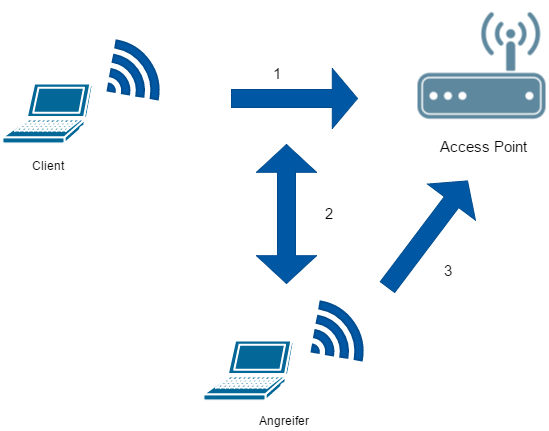
\includegraphics[width=0.7\textwidth]{bilder/wlan/WLANSzenario.png}\\

Angriffe auf ein Wireless Network laufen häufig nach einem bestimmten Schema ab. 
Dazu werden Daten, die zwischen Client und Netzwerkgerät hin- und hergeschickt werden, gesammelt. Diese Informationen werden dann beim Angreifer in einer gewissen Art und Weise verarbeitet.
Ist diese Verarbeitung, egal wie komplex diese ist, erfolgreich, so hat der Angreifer häufig Zugriff auf das Netz. 

\section{Vorbereitungen}

Voraussetzungen für die weiteren Übungen:\\

- Alfa USB WLAN-Adapter\\
- Workstation/Notebook\\
- Virtual Box mit Kali Linux Image (+ Extension Pack)\\
- Grundlegende Kenntnisse mit Linux\\

Konfiguration des Alfa Adapters in Kombination mit Virtual Box:\\

Anschluss des Adapters über das beigelegte Y-Kabel an den Host.
In Virtual Box die Kali Maschine auswählen $\rightarrow$ Rechtsklick: Ändern $\rightarrow$ USB auswählen $\rightarrow$ USB-2.0-Controller aktivieren $\rightarrow$ USB-Filter hinzufügen
$\rightarrow$ Ralink WLAN auswählen (falls nicht vorhanden im GeräteManager nach dem WLAN Adapter suchen) $\rightarrow$ Mit OK bestätigen.\\
%Zusätzlich einen neuen Filter anlegen und Hersteller- bzw. Produkt-ID aus dem ersten Filter übernehmen. Die anderen Felder können unausgefüllt werden
Den WLAN Adapter ausstecken\\

Kali Linux in Virtual Box starten (user: root, passwort: toor)\\
Sobald die VM hochgefahren ist, den Adapter einstecken.\\
USB Icon im Fenster der Maschine sollte rot/grün blinken.\\ %(evtl screenshot)\\

In einigen Fällen, kann es zu Problemen in der Kommunikation von der virtuellen Maschine zu dem Adapter kommen. 
Dann kann es helfen entweder den Adapter aus- und wieder anzustecken oder die Einstellung für das Durchreichen des USB-Adapters aus- und wieder anzuschalten.


\section{WEP}

\section{WPA/WPA2}


WPA bzw. WPA2 (WiFi Protected Access) ist eine Kombination aus Authentifizierung und Verschlüsselung, um ein WLAN sicher zu betreiben. Die Authentifizierung erfolgt in der Regel mit einem Passwort, um den Zugriff durch unberechtigte Personen zu verhindern. Möchte ein Angreifer nun in das Netzwerk eindringen, muss er dieses Passwort herausfinden.\\


Grundsätzlich gibt es beim Hacken keine Unterschiede zwischen WPA- und WPA2-gesicherte WLANs. Die Authentifizierungsmethode ist im Prinzip identisch. Der Unterschied liegt im Verschlüsselungsverfahren, welche für die typischen Hacking-Methoden auf WPA-gesicherte WLANs nicht relevant ist.\\ Grund dafür ist, dass WPA2 derzeitig noch als nicht zu knackendes Verschlüsselungsverfahren
gilt und daher ein Angriff auf die Verschlüsselung vergebene Mühe wäre. \\

Der typische Angriff gegen ein WPA-/WPA2-gesichertes WLAN läuft über reines Bruteforcing oder einer sogenannten Wörterbuch-Attacke (engl. dictionary-attack). Bei ersterem werden einfach alle Kombinationen bestehend aus Buchstaben, Ziffern und Sonderzeichen, oder nur einem Ausschnitt davon, bis zur gewünschten Länge getestet. Je nach Länge und Komplexität des Passworts kann sich dieser Vorgang über viele Stunden, bis zu Tagen und sogar mehreren Jahren hinziehen. Häufig wird bei einer Bruteforce-Attacke zuvor eine Wordlist, wie bei einem Dictionary-Angriff, mit allen zu testenden Kombinationen erstellt. Bei einem Wörterbuch-Angriff wird somit durch die Passwortkandidaten in einer riesigen Wordlist iteriert und mit dem herauszufindenden Passwort abgeglichen. %wie abgeglichen? verhasht ,bzw. verschlüsselt? 
Stimmen beide überein, wurde das Passwort gefunden. Diese Wörterlisten können entweder selber generiert werden oder sind auch im Internet zu finden. Wie wir später noch sehen werden, gibt es auch hybride Ansätze, die beide Angriffsarten verknüpfen.\\


Ein WPA-Handshake findet zwischen Access Point und WLAN-Client statt, wenn der WLAN-Client sich mit dem WLAN verbinden will. Dieser WPA-Handshake muss aufgezeichnet werden. Anschließend wird bei einem Wörterbuch-Angriff mit Hilfe der Wordlist das WLAN-Passwort erraten. Ein erfolgreicher Angriff steht und fällt mit einer guten Wordlist, in der das WLAN-Passwort enthalten sein muss. Darin besteht die eigentliche Schwierigkeit bei einem WPA/WPA2-WLAN-Hack.\\


Grober Ablauf eines WPA-/WPA2-Hacks:

\begin{enumerate}
\item Wordlist erstellen oder besorgen 
\item Grundzustand herstellen und Monitor Mode einschalten
\item WLAN mit WPA/WPA2 identifizieren (Information Gathering) 
\item Datenverkehr mit Airodump-ng aufzeichnen
\item Deauthentication-Attacke mit Aireplay-ng (optional)
\item WPA-Passwort mit Hilfe der Wordlist herausfinden
\end{enumerate}

%more space

\textbf{\Large{Cracking des WPA Keys}}\\ %(evtl mit Screenshots oder weiter ausformulieren)

{\Large 1. Check des WLAN Adapter}\\

Zuerst muss geprüft werden, ob der eingesteckte USB WLAN-Adapter erkannt wird und somit einsatzbereit ist. Dazu das Terminal öffnen in Kali Linux öffnen und folgenden Befehl eingeben. 

$$iwconfig$$\\

Der Adapter sollte als Interface, meist WLAN0 oder WLAN1, angezeigt werden\\
Im Folgenden muss bei allen Befehlen die Interface Bezeichnung mit der hier angezeigten ersetzt werden, da sie sich von Rechner zu Rechner unterscheiden kann.\\


{\Large 2. MAC-Spoofing}\\

Im Sinne von Wireless Security sollte man sich immer im Klaren sein, dass ein Angreifer immer in der Lage ist seine MAC-Adresse zu verändern. Dieser Vorgang wird auch Spoofing genannt.

Die MAC-Adresse ist eine herstellerspezifische Kennung, die fest einem Netzwerkgerät zugeordnet ist. Jede Adresse ist eindeutig. Findet man die MAC-Adresse eines Angreifers heraus, kann mit Hilfe dieser Identifikationskennung festgestellt werden, welchen Typ von Antenne er verwendet. Diese Erkenntnis kann helfen einen Angreifer zu identifizieren.
Verwendet ein Angreifer nun eine gefälschte MAC-Adresse können keine Rückschlüsse auf seine Identität gezogen werden, da überall nur seine Fake-Adresse angezeigt wird.\\

Zuerst muss dafür das WLAN Interface deaktiviert werden. Danach kann mit dem Kommando \textit{macchanger} die Adresse geändert werden.\\

\begin{equation*}
\begin{split}
ifconfig~wlanX~down\\
macchanger~\text{-}r~wlanX
\end{split}
\end{equation*}

\textit{X = NUM für das interface}\\

Beim Bestätigen des Befehls mit Enter, wird die eigene MAC-Adresse in eine zufällige generierte MAC-Adresse geändert und auf der Konsole angezeigt. Anschließend kann das Interface mit folgendem Befehl wieder aktiv gesetzt werden.\\
 
$$ifconfig~wlanX~up$$

\textit{X = NUM für das interface}\\


Mit dem Befehl\\ 
$$ifconfig~wlanX$$

\textit{X = NUM für das interface}\\

kann überprüft werden, ob die gespoofte MAC-Adresse auch aktiv ist.\\

{\Large 3. Das Interface in den Monitor Mode versetzen}\\

Damit mit dem WLAN Adapter Pakete aufgezeichnet werden können, muss sich der Adapter im Monitoring Mode, oder auch Packet Injection Mode genannt, befinden. Dies wird mit folgendem Befehl erreicht.

$$airmon\text{-}ng~start~wlanX~$$

\textit{X = your number from iwconfig}\\

Mit dem Befehl\\ 

$$airmon\text{-}ng~check~kill$$

\textit{X = NUM für das interface}\\


werden alle andere Prozesse beendet, die auch auf den Netzwerkadapter zugreifen können. So können Konflikte beim Zugriff auf die Ressource vermieden werden.\\

{\Large 4. Aufzeichnen der WLAN Pakete mit airodump}\\
	
Im nächsten Schritt werden die WLAN Pakete aus der Umgebung aufgezeichnet. Damit möchte man einen Handshake zwischen dem zu hackenden Access Point und einem Client aufzeichnen. Anhand dessen kann anschließend das Passwort herausgefunden werden.\\

Mit dem folgenden Befehl können wir in den Aufzeichnungsmodus umschalten.
	
	$$airodump\text{-}ng~\text{-}b~a~wlanXmon$$\\
	 
	\textit{X = NUM für das interface}\\
	\textit{-b a = Scan im 5GHz Band}\\	
	
Falls wir im im 5GHz Bereich scannen möchten muss der Parameter \textit{-b a} mitgegeben werden. Falls nicht, kann der Parameter einfach weggelassen werden.\\	
Sollten keine Daten aufgezeichnet werden, dann den Adapter mehrmals aus- und wieder einstecken. 
Nach einem Reconnect muss der Adapter natürlich wieder in den Monitoring Modus versetzt werden.
	
Hat alles soweit geklappt, sollten alle erreichbaren SSIDS mit ihren jeweiligen Sendern angezeigt werden.\\ 
	
Als nächstes sollte die MAC-Adresse und der verwendete Kanal des zu hackenden APs notiert.
Anschließend kann durch einen neuen airodump-ng Durchlauf mit der MAC und dem Kanal als Parameter (nähere Infos unter \(man~airodump-ng\) abrufbar) der Scan
	eingeschränkt werden. Zusätzlich kann auch der Name der Ausgabedatei festgelegt werden. 
Der Befehl sieht dann in etwa wie nachfolgend aus.
	$$airodump\text{-}ng~\text{-}c~Kanal~\text{-}b~a~\text{-}\text{-}bssid~MAC\text{-}AP~\text{-}showack~\text{-}w~Filename~wlanXmon$$
	
		\textit{X = NUM für das interface}\\
		\textit{Kanal = der Kanal auf dem gelauscht werden soll}\\
		\textit{MAC-AP = die MAC-Adresse des Access Points}\\
		\textit{Filename = in die zu schreibende Datei}\\

	Verbindet sich nun ein Client auf den AP, so kann der 4-way-handshake mitgelesen werden, was auch in der Konsole, in der rechten oberen Ecke, angezeigt wird.
	Hat dies funktioniert, ist der erste Schritt für das Hacken des Passworts abgeschlossen.\\

{\Large 5. Cracken des Passworts}\\
		
Ab hier werden verschieden Tools und Angriffsarten für das Cracken des Keys vorgestellt.\\	

 \textbf{Dictionary Attack mit aircrack}\\

Dazu wird ein Dictionary File mit allen Passwörtern benötigt, die auf Übereinstimmung mit dem PSK gecheckt werden sollen. Auf dem Image sollt bereits eine Dictionary Datei im Home Verzeichnis vorhanden sein.

Mit folgendem Befehl kann der Dictionary-Angriff gestartet werden. 

$$aircrack\text{-}ng~\text{-}w~dict.file~\text{-}b~MAC\text{-}AP~File.cap$$

\textit{dict.file = Pfad zu dem Dictionary}\\ 
\textit{MAC-AP = Die MAC-Adresse des APs}\\ 
\textit{File.cap = Pfad zu dem cap file}\\

\textbf{Brutefore Angriff mit aircrack und crunch}

\begin{equation*}
\begin{split}
crunch~8~12~abcdefghijklmnopqrstuvwxyzABCDEFGHIJKLMNOPQRSTUVWXYZ \\
|~aircrack\text{-}ng~\text{-}\text{-}bssid~00:11:22:33:44:55~\text{-}w\text{-}~hack\text{-}wifi\text{-}01.cap
\end{split}
\end{equation*}
 
\textit{8 12 = die zu testende Passwortlängen, hier von Länge 8 bis 12}\\
\textit{abcde.. = die zu testenden Zeichen}\\



\textbf{Attacken mit hashcat}\\

Bei hashcat handelt es sich wohl um den derzeit schnellsten Passwortcracker auf dem Markt. Wir verwenden es als Alternative zu crunch.\\

Convert the .cap file in a hccap file\\

$$aircrack\text{-}ng~Filename.cap~\text{-}J~newFilename$$

\textit{Filename.cap = Pfad bzw. Name des alten .cap files}\\
\textit{Pfad bzw. Name des neuen .hccap file}\\

%+ Brutefore/Dictionary/Rule-Based Attack with hashcat möglich

Mit hashcat --help kann eine Hilfeseite aufgerufen werden in welcher der Befehl, die Parameter und die Verwendung
genauer erläutert werden. Falls Probleme auftreten oder detailliertere Einstellungen vorgenommen werden sollen, kann 
die Hilfeseite die erste Anlaufstelle sein.\\

\textbf{Dictionary Attack mit hashcat}

$$hashcat~\text{-}m~2500~capture.hccap~dict.txt$$\\

\textit{-m 2500 = Anweisung, dass ein WPA/WPA2 Key gecrackt werden soll}\\
\textit{caputre.cap = Pfad bzw. Name des hccap file}\\
\textit{dict.txt = Pfad bzw. Name des dictionary file}\\

Anschließend nutzt hashcat das Dictionary um das Passwort zu finden.
Mit Enter kann der aktuelle Status des Vorgangs abgefragt werden.\\ 

\textbf{Bruteforce Attack mit hashcat}

$$hashcat~\text{-}m~2500~\text{-}a3~capture.hccap~?d?d?d?d?d?d?d?d~(?d = 0\text{-}9)$$

\textit{-m 2500 = Anweisung, dass ein WPA/WPA2 Key gecrackt werden soll}\\
\textit{-a3 = Verwende Bruteforce}
\textit{caputre.cap = Pfad bzw. Name des hccap file}\\
\textit{?d..?d = definierte Maske für zu testenden Passwortkandidaten, Anzahl entspricht "bis zu Länge"\\
Weitere Optionen:\\
?l = abcdefghi...yz\\
?u = ABCDEFGHI...YZ\\
?s = Sonderzeichen\\
?a = ?l?u?s?d}\\

Bei der Bruteforce Attacke werden alle Kombinationen von Buchstaben bis zu einer bestimmten Länge durchgetestet.
Als letzter Parameter kann eine Art Maske angegeben werden, mit welcher die Länge und die zu testenden Ziffern, Buchstaben
und Zeichen festgelegt werden. Im Beispiel werden alle bis zu neunstelligen Zahlenkombinationen von hashcat durchprobiert.\\ 

\textbf{rule-based Attack mit hashcat}

$$hashcat~\text{-}m~2500~\text{-}r~/usr/share/hashcat/rules/best64.rule~capture.hccap~ dict.txt$$\\

\textit{-m 2500 = Anweisung, dass ein WPA/WPA2 Key gecrackt werden soll}\\
\textit{-r Pfad zum rules file = Verwende rule-based Angriff und Pfad}\\

rule-based attacks gehören zu den komplizierteren Angriffsarten. Dabei wird ein nomaler Dictionary-Angriff gefahren, aber mit rules erweitert. 
Die rules, zu deutsch Regeln, sind wie eine Art Programmiersprache
für die Generierung von Passwörtern. Es gibt Funktionen mit denen Passwortkandidaten bearbeitet, mit anderen Wörtern verknüpft oder bestimmte Kombinationen 
übersprungen werden können. Regeln zu schreiben kann sehr aufwendig sein und erfordert viel Wissen über Passwörter. Daher kann für die ersten Versuche auch 
die best64.rule Regel verwendet werden, die standardmäßig bei hashcat dabei ist.\\


%DoS Attack mit MDK3

%Erst den Adapter wieder in den Monitoring Mode versetzen.

%airmon-ng start wlanX

%disconnect bei verwendung von mdk3

\textbf{Cracking des Passworts mit Hilfe der Grafikkarte}\\

Neben dem normalen Hashcat gibt es eine weitere Version, die sich oclHashcat nennt. Mit dieser Version ist es möglich das Cracken Keys mit Hilfe der Grafikkarte durchzuführen. Hierfür sind die Geschwindigkeiten stark von der Leistungsfähigkeit der verwendeten Grafikkarten abhängig. 
Jedoch sind deutliche Leistungssteigerungen gegenüber der CPU in den meisten Fällen, bei halbwegs aktueller Hardware, zu erwarten. Notwendig sind aktuelle Treiber, die auf dem System installiert sein müssen. Weitere Infos dazu gibt es auf der Homepage von oclHashcat. 
Weiter ist es möglich mehrere Grafikkarten im Clusterbetrieb parallel für das Cracken eines Keys zu betreiben. Dadurch können noch größere Performancesteigerungen erzielt werden.

Leider ist es nicht möglich oclHashcat aus der virtuellen Maschine heraus zu verwenden, da der direkte Zugriff auf die Grafikkarte verweigert wird. Das Cracken per GPU kann hier deshalb nur exemplarisch beschrieben werden. Natürlich steht es jedem frei, mit dem hier gezeigten Verfahren auch zu Hause auf seinem privaten Rechner zu experimentieren.\\

\textit{Anwendungsfall}\\

Als Anwendungsfall wollen wir die Standard WLAN Keys von den Herstellern untersuchen. Oft werden von diesen längere Zahlenketten als default gesetzt. Natürlich könnte der Vergleich von CPU zu GPU auch mit anderen Passwörtern durchgeführt werden. 

In unserem Beispiel (FritzBox) ist vom Hersteller aus eine 16-stellige Ziffernfolge als Key gesetzt. Das Wissen, dass es sich nur um Ziffern handelt kann später beim Cracken ein deutlicher Vorteil sein.

Zuerst wird, wie in den oberen Kapiteln der Handshake zwischen dem Access Point und einem Client aufgezeichnet. Anschließend muss das aufgezeichnete .cap File für hashcat wieder in ein .hccap File umgewandelt werden. Wie dies funktioniert ist in den vorherigen Kapiteln bereits beschrieben worden. \\

Im nächsten Schritt soll einmal mit der CPU und einmal mit der GPU der Key herausgefunden werden. Dazu wird hashcat für den Durchlauf auf dem Prozessor und einmal oclHashcat, eine spezielle Version für die GPU, verwendet.\\ 

\textit{Durchführung 1}\\

Der erste Versuch wird wieder mit hashcat ausgeführt. Dazu wird der Befehl wie in dem vorhergehenden Kapiteln verwendet. Wir wissen nun aber, dass der Schlüssel eine Länge von 16 Zeichen besitzt und wir somit die Längen 1 - 15 nicht testen müssen. Dazu wird der Befehl um einen weiteren Parameter, der die einzige zu testende Länge angibt, erweitert.
%stimmt der befehl so??
$$hashcat~\text{-}m~2500~\text{-}a3~capture.hccap~\text{-}\text{-}pwd\text{-}min\text{=}16~?d?d?d?d?d?d?d?d~(?d = 0\text{-}9)$$\\

\textit{-m 2500 = Anweisung, dass ein WPA/WPA2 Key gecrackt werden soll}\\
\textit{-a3 = Verwende Bruteforce}
\textit{caputre.cap = Pfad bzw. Name des hccap file}\\
\textit{?d..?d = definierte Maske für zu testenden Passwortkandidaten, Anzahl entspricht "bis zu Länge"\\}\\


Die folgende Abbildung zeigt die Ausgabe sobald mit Enter der Befehl bestätigt wurde.\\

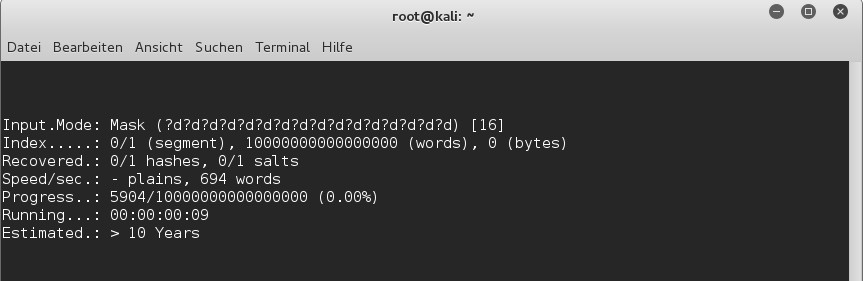
\includegraphics[width=\textwidth]{bilder/wlan/wlan_screenshot_1.png}\\

Dort sind einige interessante Informationen zu dem Durchlauf zu sehen. Die Geschwindigkeit beträgt knapp 700 Wörter pro Sekunde und dürfte sich für die meisten Prozessoren in diesem Bereich bewegen.
Als wichtigste Info wird die geschätzte Zeit für das Cracken betrachtet. Man sieht, dass hier mehr als 10 Jahre angenommen werden. Dies ist auch nicht weiter verwunderlich, wenn man den Blick auf die riesige Anzahl an Kombinationsmöglichkeiten richtet. Selbst durch die genaue Länge und dem Wissen, dass es sich nur um Zahlenkombinationen handelt konnte die Laufzeit nicht auf ein erträgliches Maß gesenkt werden. Somit ist das Cracken des Keys nicht mit einem einzelnen Prozessor und wohl auch nicht mit einer kleinen Anzahl an Rechenwerken möglich.\\

\textit{Durchführung 2}\\

Dieselbe Berechnung soll nun auf der Grafikkarte durchgeführt werden. Dazu wird oclHashcat verwendet, welches kostenfrei von deren Website heruntergeladen werden kann. Das Tool wird einfach entpackt und je nach Betriebssystem über die Kommandozeile gestartet. Der Befehl auf einem Windows System sieht folgendermaßen aus und ähnelt sehr stark dem vorherigen Aufruf.

$$cudaHashcat64.exe~\text{-}m~2500~\text{-}a~3~capture.hccap~\text{-}pwd\text{-}min\text{=}16~?d?d?d?d?d?d?d?d~(?d = 0\text{-}9)$$

\textit{-m 2500 = Anweisung, dass ein WPA/WPA2 Key gecrackt werden soll}\\
\textit{-a 3 = Verwende Bruteforce}
\textit{caputre.cap = Pfad bzw. Name des hccap file}\\
\textit{?d..?d = definierte Maske für zu testenden Passwortkandidaten, Anzahl entspricht "bis zu Länge"\\}\\

Wurde der Befehl bestätigt, kann mit der Taste "s" der Status des Vorgangs eingesehen werden. Einige Dinge sind bereits aus dem vorherigen Aufruf bekannt. Interessant sind die Keys per second, die getestet werden. Der Wert liegt hier bei 41586. Somit liegt der Speedup im Vergleich zur CPU bei fast 60facher
Geschwindigkeit. Dies ist natürlich deutlich schneller als im vorherigen Durchlauf. Jedoch wird auch in diesem Fall eine geschätzte Zeit von über 10 Jahren angezeigt. Das bedeutet, dass trotz der besseren Performance keine signifikante Verringerung der Laufzeit erreicht wurde. 
Letztendlich kann nun auch mit einer einzelnen GPU dieser Standard Key nicht geknackt werden.\\

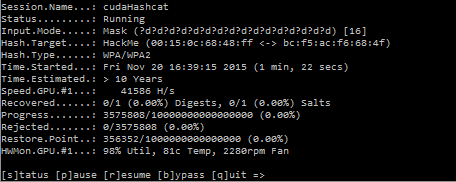
\includegraphics[width=\textwidth]{bilder/wlan/cudaHashcatNUMSeriesCrack.png}\\

%evtl noch Diagramm hier


\section{WPS}

Falls alle vorherigen Angriffe gegen ein WPA/WPA2 gesichertes Netzwerk fehlgeschlagen sind, kann ein weiterer spezieller Angriff durchgeführt werden. Dieser Angriff kann durchgeführt werden, falls WPS (Wi-Fi Protected Setup) auf dem anzugreifenden Netzwerkgerät aktiviert ist. Das Netz kann so gehackt werden, ohne den PSK direkt anzugreifen. WPS wurde entwickelt um das Hinzufügen von Geräten zu einem Netzwerk zu vereinfachen ohne die Sicherheit der Verschlüsselung zu umgehen. Dazu stehen verschiedene Modi zur Verfügung. Zwei davon sind sehr beliebt. Zum Einen kann über die Eingabe eines PIN, der fest in dem Gerät hinterlegt ist ein Client hinzugefügt werden. Bei der zweiten Variante musst WPS auf dem Client als Verbindungsmethode gewählt werden und gleichzeitig wird dazu ein Hardware Button auf dem Netzwerkgerät gedrückt. Bei diesem Hack wird der feste 8-stellige PIN angegriffen. \\

Bei 8 Stellen gibt es 100.000.000 verschiedene Kombinationen. Zu unserem Glück kann durch das Ausnutzen von Lücken in dem Standard der Aufwand auf 11.000 Kombinationen eingegrenzt werden. Zieht man einige Statistiken zu Rate, dann zeigen diese, dass das Cracken des WPA/WPA2 Passworts statistisch gesehen im Durchschnitt in der Hälfte der Zeit dieses Angriffes durchgeführt werden kann. Natürlich gibt es keine Garantie dafür. Weshalb dieser Angriff auf WPS auf jeden Fall erwähnt werden sollte. 

Um diesen Angriff auszuführen, wird wie bei den anderen Angriffen meist auch der WLAN Adapter vorbereitet.\\

Dieser wird zu Beginn mit nachfolgendem Befehl in den Monitoring Mode versetzt.\\

$$airmon\text{-}ng~start~wlanX~$$

\textit{X = NUM für das interface}\\


Anschließend werden wieder mit airodump die Pakete aufgezeichnet. \\

$$airodump\text{-}ng~\text{-}b~a~wlanXmon$$\\
	 
	\textit{X = NUM für das interface}\\
	\textit{-b a = Scan im 5GHz Band}\\	

In der angezeigten Liste den anzugreifenden Access Point identifizieren. Von diesem wird im Weiteren die MAC Adresse(BSSID) benötigt.
Mit Strg+C kann nun das Aufzeichnen wieder beendet werden. Ab hier kann der WPS Angriff gestartet werden. Dazu wird das Cracking Tool Reaver verwendet. Dieses kleine Programm versucht den WPS PIN des Access Points herauszufinden. Voraussetzung für den Angriff ist natürlich, dass WPS auf dem Target aktiviert ist. \\

Der Befehl sieht dann wie folgt aus:\\


$$reaver~\text{-}i~wlanXmon~\text{-}b~MAC\text{-}AP$$

\textit{X = NUM für das interface}\\ 
\textit{MAC-AP = Die MAC-Adresse des APs}\\ 

Nun sollte Reaver den beginnen den 8-stelligen PIN zu knacken. Dieser Vorgang dauert zwischen 4 und 5 Stunden. Im Gegensatz zum Cracken eines WPA/WPA2 Passworts, wird hier der PIN garantiert gefunden, was einen deutlichen Vorteil darstellt. \\

\textit{Troubleshooting:}\\

Beim WPS PIN cracken kann es in Einzelfällen zu Timeouts oder anderen Fehlern kommen. Oft hilft es danach zu googlen, da dies sehr spezielle Ursachen haben kann. \\

Wird nach ca. 10 Versuchen eine Warnung angezeigt, kann es sein, dass der AP die Connections limitiert, falls er zu viele Anfragen bekommt. Oder er kommt mit der Vielzahl an Anfragen nicht zurecht. In diesen Fällen kann eine kurze Wartezeit zwischen den Anfragen weiter helfen. Dazu den obigen Befehl mit dem Parameter\\

$$\text{-}fail\text{-}wait\text{=}300$$\\

erweitern. Der Wert muss nicht fest sein, sonder kann variiert werden um optimale Ergebnisse zu erzielen. 



\section{Sicherungsmaßnahmen und Bewertung}

Nachdem nun die gängigsten Angriffsarten und ihre Durchführung erläutert wurden, soll hier abschließend eine kurze Bewertung abgegeben werden. Wie in den ersten Sektionen des Kapitels zu erkennen ist, bietet WEP als Verschlüsselung keinen nennenswerten Schutz mehr und kann ohne viel Aufwand geknackt werden. Daher ist es ratsam nur noch WPA2, da WPA ebenfalls bereits veraltet ist, zu verwenden. Zu beachten ist dabei, einen ausreichend langen und komplexen Key zu hinterlegen. Solange es keine Schwachstelle in der Umsetzung des Herstellers gibt, ist der Schlüssel der einzige Angriffspunkt auf die WPA2 Verschlüsselung. \\

Weiter wurde gezeigt, dass WPS eine weitere Schwachstelle darstellt und ein Angreifer so die Sicherheit einer starken Verschlüsselung vollkommen umgehen kann. Daher ist es ratsam WPS nur in Ausnahmefällen zu verwenden und ansonsten dieses Feature zu deaktivieren. \\

Ein weit verbreiteter Irrtum ist auch, dass das Verstecken des Netzwerknamens, auch SSID genannt, die Sicherheit verbessert. Jedoch haben wir gesehen wie einfach nach WLAN Netzwerken in der Umgebung gescannt werden kann. Dabei alle Netzwerke, auch diejenigen mit versteckter SSID, angezeigt. Damit verbessert dieses Feature, was viele Netzwerkgeräte unterstützen, definitiv nicht. 



	
	%Kapitel zum iCTF
	\chapter{UCSB International Capture The Flag}
In diesem Kapitel wird auf den Hacker-Wettbewerb UCSB International Capture The Flag (iCTF) eingegangen. Zuerst wird Allgemeines dazu erläutert. Anschließend wird der zu erstellenden Service beschrieben. Im letzten Abschnitt wird anschließend auf die Durchführung des Wettkampfes eingegangen.

\section{Allgemeines}
Der iCTF wird jährlich von der University of California, Santa Barbara (USCB) veranstaltet und ist der größten Hackerwettbewerbe dieser Art. 
Der iCTF integriert Angriff und Verteidigung zugleich. Die Teilnehmer müssen gleichzeitig Flaggen von fremden Servicen erhalten, sowie ihre eigenen Service patchen um diese nicht mehr angreifbar zu machen.

\section{Service}
In diesem Abschnitt wird der Service für den iCTF erläutert. Dazu wird zuerst auf die Anforderungen eingegangen. Danach wird die Idee beschrieben. Zuletzt wird der Aufbau und die grundlegende Umsetzung dargestellt

\subsection{Anforderungen}
Zuerst mussten die Anforderungen für den Service definiert werden. Dazu wurden neben den offiziellen Anforderungen seitens der USCB auch eigene Anforderungen vom Projekt Team entworfen.

Um einen Service erfolgreich beim iCTF einreichen zu können mussten verschiedene Punkte beachtet werden:

\begin{enumerate}
\item Es muss eine Service angeboten werden, welcher dem Benutzern eine Funktion anbietet. Hier wurden in einem früheren Wettbewerb zum Beispiel ein Service zum Überprüfen der Temperatur angeboten.
\item Ein weiterer Punkt war die Benutzerinteraktion. Hier wurden den Team zwei Möglichkeiten gegeben. Entweder kann auf den Service über ein Webinterface zugegriffen werden oder über die Konsole.
\item Der Service muss zudem eine Sicherheitslücke besitzen, über welche eine Flag ausgelesen werden kann. 
\item Der letzte Punkt beschreibt das Thema für den aktuellen iCTF. Was dieses Jahr (2015) crowdsourcing evil war.
\end{enumerate}

Weiter wurden auch vom Team Anforderungen an den Service gestellt:
\begin{enumerate}
\item Der Service soll zwei Sicherheitslücken aufweisen. Dadurch wird der Schwierigkeitsgrad und die Dauer erhöht welche zum Hacken benötigt wird.
\item Eine weitere Anforderung seitens des Teams bestand darin, dass der Service eine lustige Funktion bieten soll.
\item Zuletzt sollten der Service möglichst leicht umgebaut werden können, dass er auch für die Lehre an der Technische Hochschule verwendet werden kann.
\end{enumerate}


\subsection{Idee}
Für den Service wurden zu Beginn verschiedene Ideen diskutiert. Dabei wurde zunächst auf die Funktion des Services eingegangen. Dabei wurden verschiedene Ansätze eingebracht:

\begin{itemize}
\item Labyrinth in einer Bibliothek
\item Kryptologie Aufgaben 
\item Abgaswerte des Volkswagen Konzerns
\end{itemize}

Aus aktuellem Anlass wurde  der letzte Punkt für den Service gewählt.

Hierbei soll ein Konsolen-Service erstellt werden, welcher die Möglichkeit bietet die Fahrgestellnummer zu überprüfen und dem Benutzer gegebenenfalls seinen Abgaswert mitzuteilen. Zudem wurde der Name des Konzerns abgeändert in Folkswagen.
\\

Als weitere Idee wurde angetragen, dass der Service in bayrischem Dialekt benutzt werden soll. Um den internationalen Teilnehmern am iCTF eine Möglichkeit zu geben den Service zu nutzen wurde zudem ein Übersetzer von Bayrisch auf Deutsch angeboten. 

\subsection{Aufbau}
Der Service wurde in zwei Teile aufgeteilt. Der erste Teil behandelt die Überprüfung der Fahrgestellnummer, der andere den Übersetzer.

\begin{figure}[H]
\centering
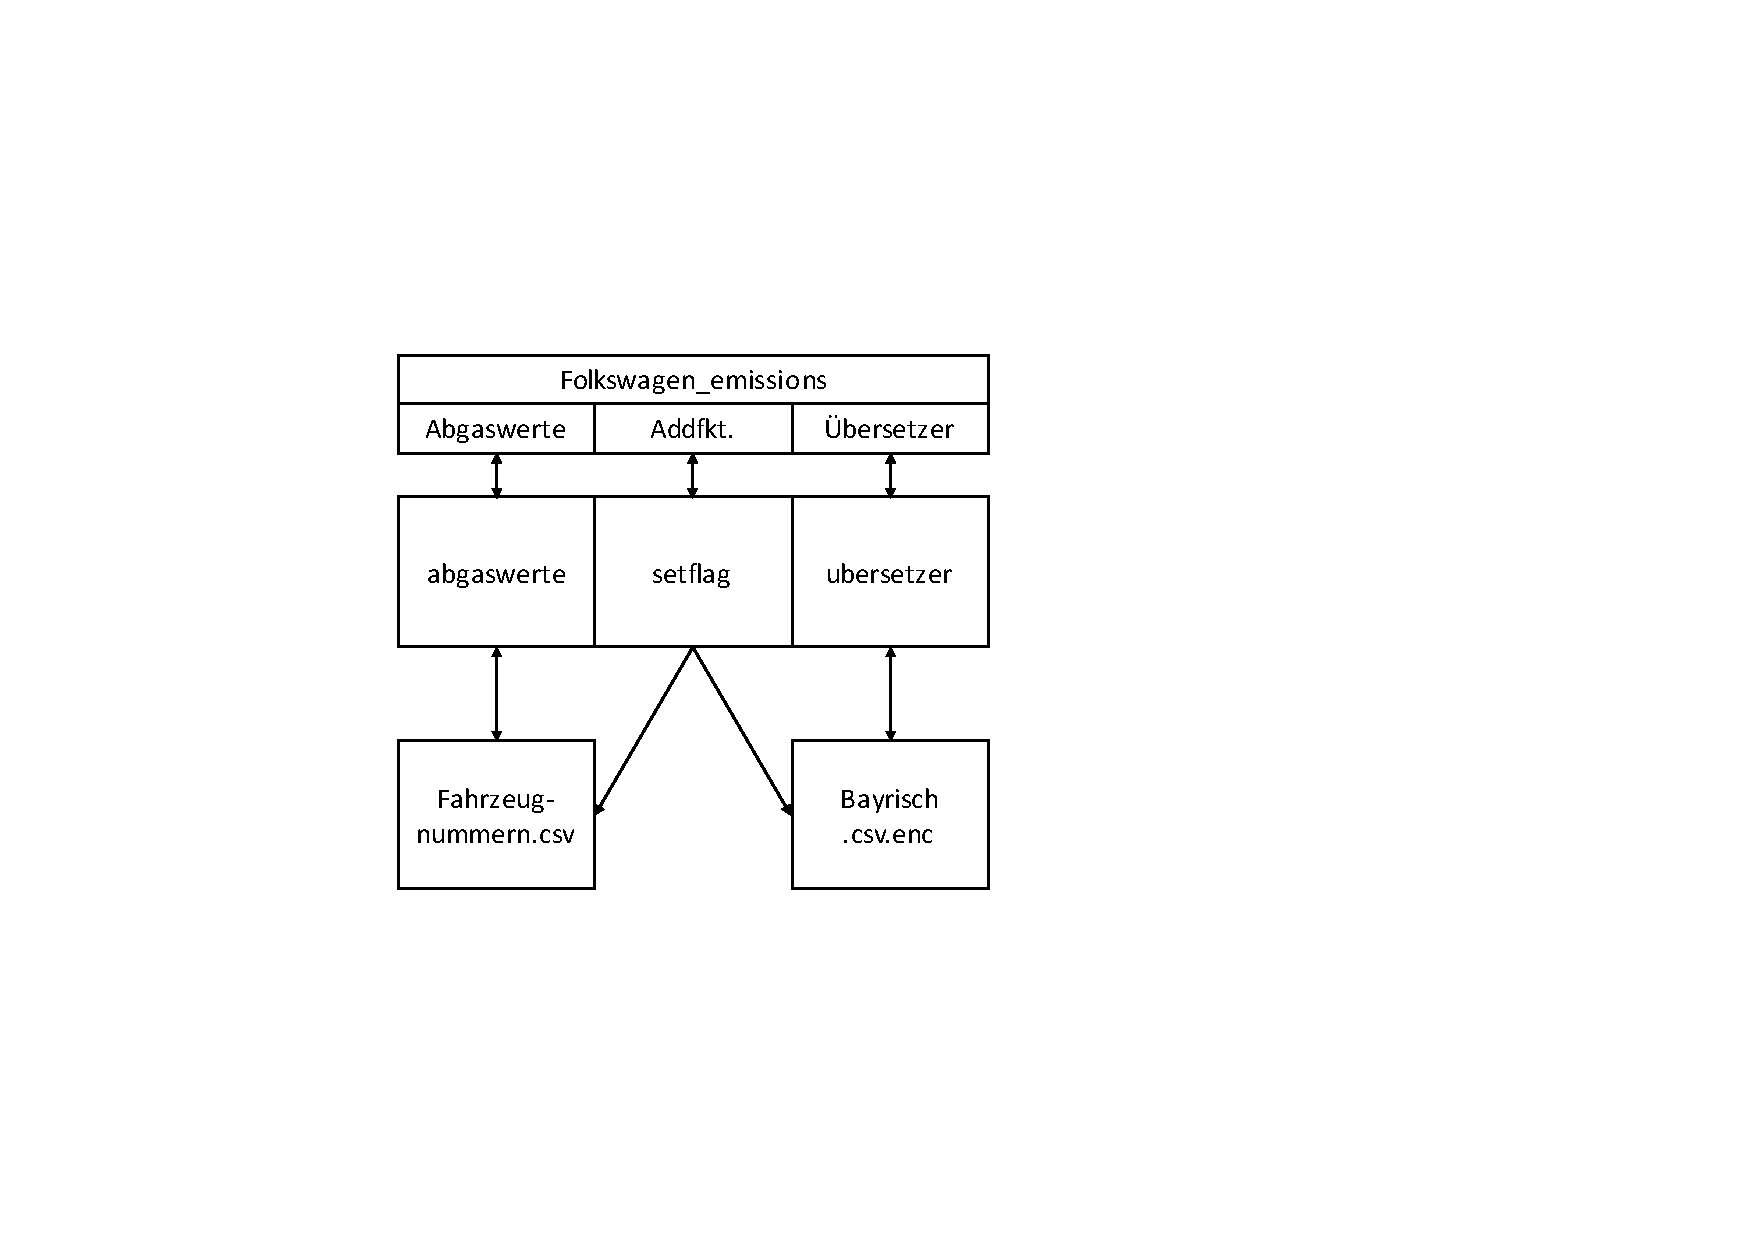
\includegraphics[scale=1]{bilder/ictf/Aufbau_Service.pdf}%
\caption{Service Aufbau}%
\label{serviceAufbau}%
\end{figure}


In Abbildung \ref{serviceAufbau} wird der zweiteilige Aufbau deutlich. Zudem wird das setzen von Flags modelliert. Hierbei handelt es sich um Funktionen für die Organisatoren, welche damit Flags setzen können.
\\

In der linken Hälfte wird der Subservice für die Fahrgestellnummer abgebildet. Dabei wird von der Konsole auf ein Modul \glqq abgaswerte\grqq zugegriffen. Dort werden mithilfe von verschiedenen csv-Dateien die Inhalte der Fahrgestellnummer verarbeitet (Zur Vereinfachung der Darstellung \ref{serviceAufbau} wurden nicht alle csv-Dateien eingezeichnet). Mithilfe dieser Daten kann die Logik entscheiden ob, eine Fahrgestellnummer richtig eingegeben wurde und gibt dann gegebenenfalls einen Abgaswert zurück. \\
Bei dieser Eingabe wird auch die erste Sicherheitslücke implementiert.
\\

In der rechten Hälfte wird der Übersetzer beschrieben. Hierbei wird wiederum über die Konsole auf die Logik zugegriffen. Der Unterschied hierbei ist allerdings, dass der Übersetzer auf eine verschlüsselte Datei zugreift. Diese wurde zum Schutz im voraus vom Projekt-Team entschlüsselt, um sicherheitsrelevante Daten zu schützen und somit die Schwierigkeit des Services zu erhöhen. Beim Zugriff auf die Übersetzungsfunktion wird das csv-File decrypted und das Wort wird in deutscher Sprache zurückgegeben. \\
Auch bei der Eingabe eines bayrischen Wortes ist eine Sicherheitslücke umgesetzt.
\\

Für das Encrypten wurde auch ein eigenes Programm entwickelt. Dieses ist jedoch nicht Bestandteil des Services sondern wurde im Vorfeld entwickelt und verwendet.

\subsection{Sicherheitslücken}
In diesen Abschnitt werden die beiden Sicherheitslücken erläutert. 

\begin{figure}[H]
\centering
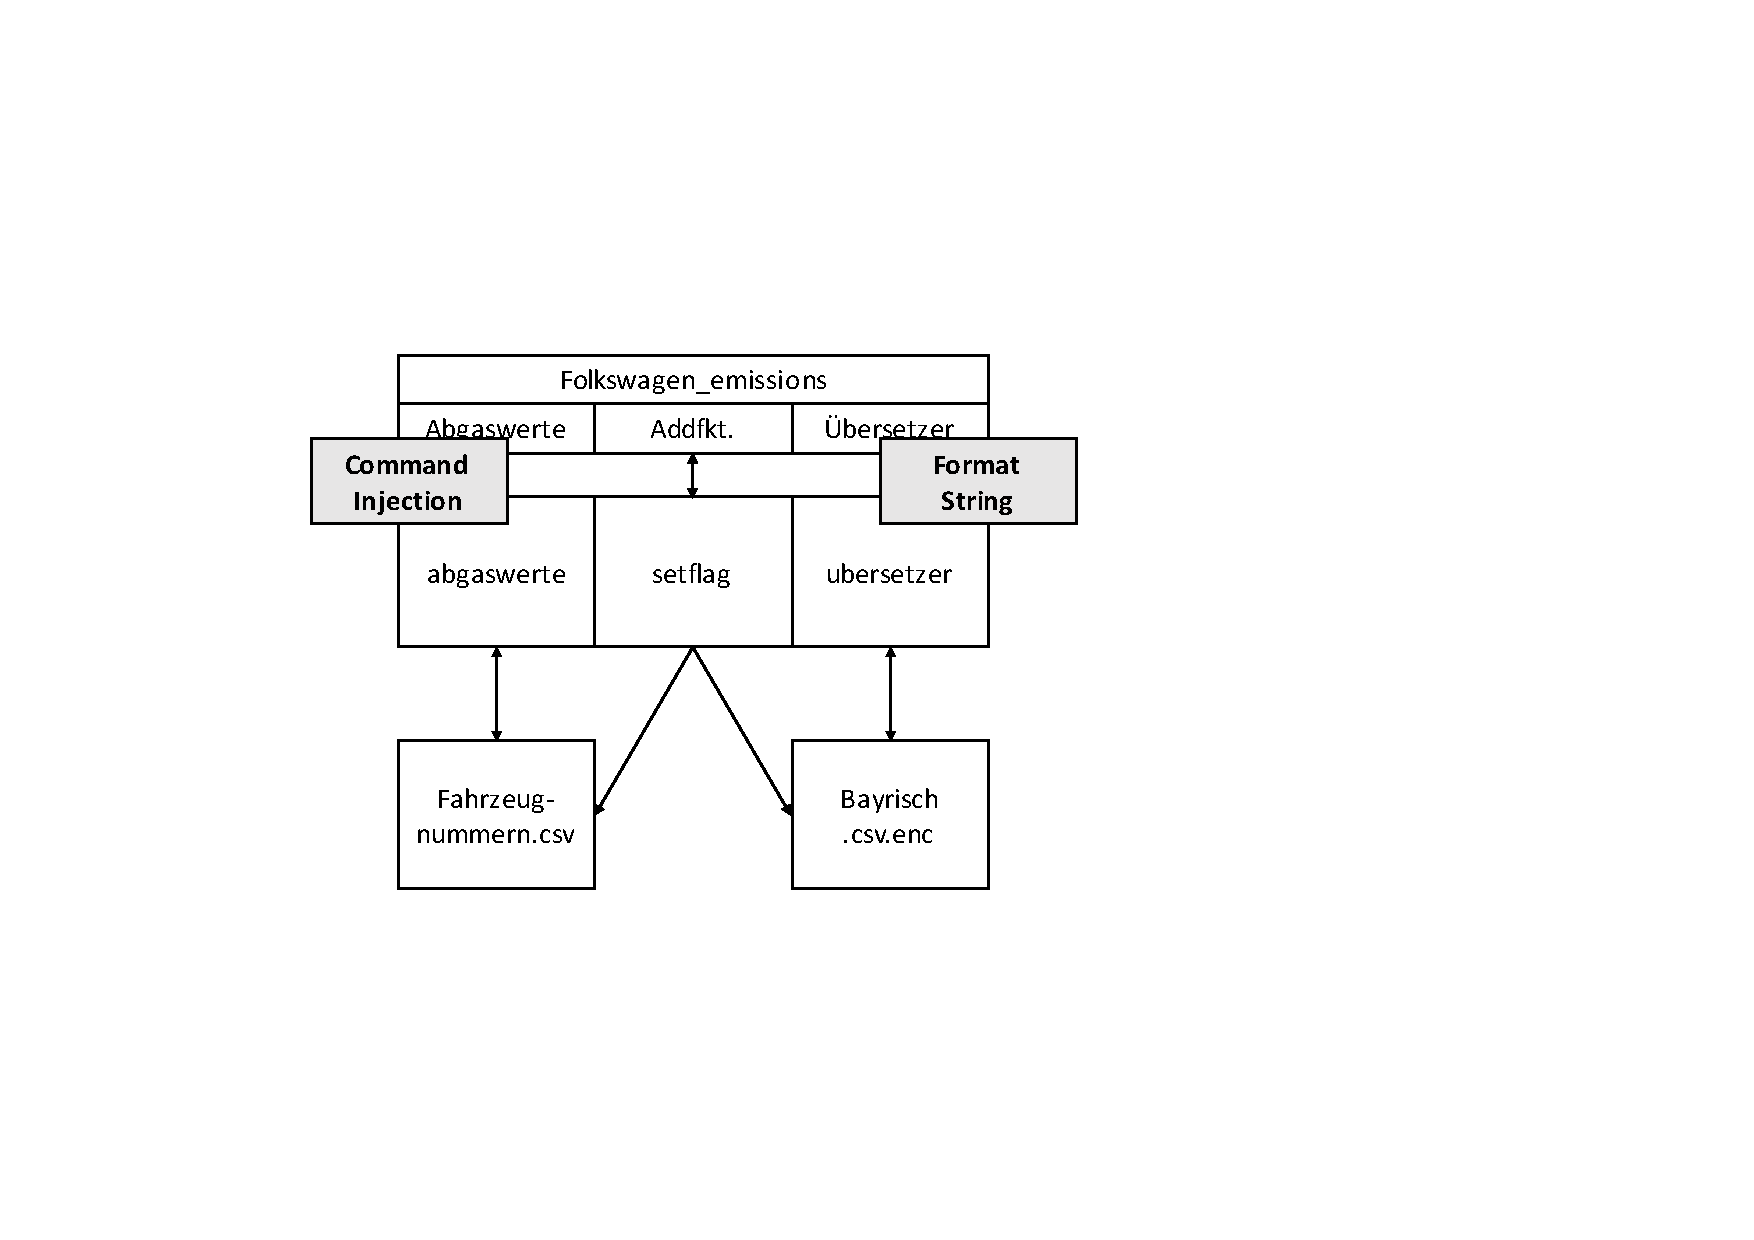
\includegraphics[scale=1]{bilder/ictf/Aufbau_Service_Luecken.pdf}%
\caption{Service Aufbau mit Sicherheitslücken}%
\label{serviceAufbauLuecken}%
\end{figure}

Wie in der Abbildung \ref{serviceAufbauLuecken} zu sehen ist, wurden in jedem Subservice eine Sicherheitslücke eingebaut. 

\subsubsection{Command Injection - Abgaswerte}
Im Abgas Teil wurde eine Command Injection eingebaut. Mithilfe dieser Sicherheitslücke kann auf was Dateisystem zugegriffen werden.
Da die Eingabe direkt auf dem Betriebssystem ausgeführt wird kann durch anhängen von Konsolen-Kommandos im Zielsystem navigiert und agiert werden. 
Dies kann durch unterschiedliche Pattern erzwungen werden:
\begin{itemize}
\item |
\item || 
\item ; 
\item \&\& 
\end{itemize}

All diese Pattern führen die angehängten Befehle aus und geben den Inhalt zurück. Dadurch kann über das Dateisystem auf die Fahrzeugnummern.csv zugegriffen und der Inhalt ausgelesen werden. 

\subsubsection{Formatstring-Angriff - Übersetzer}
Der Übersetzer wurde mithilfe von Formatstring angreifbar gemacht. Dabei können Informationen welche auf dem Stack liegen ausgelesen werden.
Um diese Lücke zu benutzen, muss im Übersetzer mithilfe der Token \%x oder \%s der Speicherinhalt auf der Konsole ausgegeben werden. Die Ausgabe muss anschließende nur noch umgewandelt werden. Somit kann hier der Inhalt der encrypteten Bayrisch.csv ausgelesen werden.
\\

Mithilfe dieser Informationen kann nun eine Flag erzeugt und beim Veranstalter eingereicht werden.
\subsection{Umsetzung}
Zuletzt wird auf die Umsetzung eingegangen. Dabei müssen drei Teile betrachtet werden. Die Oberfläche, die Abgaswerteprüfung und er Übersetzer. Zudem wird auf Umsetzung sonstiger Files eingegangen.

\subsubsection{Oberfläche}
Da die Oberfläche eine einfache Konsole ist wurde hierzu ein Python Skript entworfen, welches einen Socket implementiert. In diesem Skript wird die Interaktion mit dem Benutzer modelliert. Durch eingaben in die Konsole kann der Nutzer sich durch die verschiedenen Funktionen navigieren. So kann er zum Beispiel über den Befehlt \glqq I ko koa bayrisch\grqq  den Übersetzer starten.

\subsubsection{Abgaswerte}
Als nächstes wird auf die Umsetzung der Abgaswerteprüfung eingegangen. Dafür wurde ein C-Programm entwickelt. Die Programmiersprache C wurde gewählt, da dadurch der Code nicht eingesehen werden kann. 
\\

Bei dieser Funktion wird als Eingabe eine Fahrgestellnummer erwartet. Diese wird anschließend überprüft ob diese richtig ist. Stimmt sie mit dem Pattern überein wird ein Abgaswert aus der Fahrzeugnummern.csv ausgelesen. 
Wird eine Command Injection ausgeführt, werden hier zudem die Pattern gefiltert und der Zugriff kann ausschließlich durch \glqq \&\&\grqq durchgeführt werden.

\subsubsection{Übersetzer}
Zuletzt wird der Übersetzer beschrieben. Auch hier wurde aus den gleichen Gründen wie bei den Abgaswerten ein C-Programm entwickelt.
\\

In diesem Modul wird ein bayrisches Wort übergeben und anschließend verarbeitet. Dazu wird zunächst die encryptete Bayrisch.csv-Datei decryptet. Dabei wird der Inhalt auf den Stack geschrieben, was Grundlage für den Zugriff auf die Informationen ist. Anschließend wird überprüft, ob das Wort übersetzt werden kann. Ist dies der Fall, wird das deutsch Wort an den Benutzer zurückgegeben.

\subsubsection{Sonstiges}
Es wurden auch noch weitere Files angelegt. 
Dazu gehören unter anderem die setFlag und getFlag Funktionen. Diese wurden vom Veranstalter gefordert und verwalten die Verteilung der Flags an die Teilnehmer.
\\

Des weiteren wurde ein Exploit für den eigenen Service geschrieben welcher. Mit diesem Skript ist es möglich den Service automatisiert anzugreifen. Dadurch kann zudem einfach nachvollzogen werden welche Schritte gemacht werden müssen um an die Flag zu gelangen. Auch dieses File musste beim Veranstalter eingereicht werden.
\\

Zuletzt wurden noch csv-Datein erstellt, welche die Inhalte des Übersetzers, der Fahrgestellnummer und der Abgaswerte speichern. Diese werden von dem jeweiligen Subservice genutzt.


\section{Der iCTF 2015}
In diesem Kapitel wird auf den iCTF 2015 eingegangen. Dazu wird zuerst Allgemeines vom Event berichtet. Anschließend werden auf die Lessons Learned eingegangen.

\subsection{Allgemeines}
Dieses Jahr fand der Wettbewerb am 04.12. statt und ca. 40 Teams nahmen daran Teil. Dabei belegte unser Team (in23canation) den 22. Platz. Die Dauer des Wettbewerbs wurde mit 24 Stunden angekündigt jedoch kurz vor dem iCTF auf 8 Stunden reduziert. 
Die Stimmung beim Wettbewerb war durchgehend positiv und insgesamt war der CTF ein großer Erfolg. Durch etwas Werbung vorab war es möglich eine große Teilnehmerzahl aus allen Semestern zu begeistern sich unserer Gruppe anzuschließen. Schon bei den zwei vorangehenden Informationsveranstaltungen waren über 60 Studenten anwesend. Beim iCTF selber waren rund 25 Teilnehmer aktiv dabei. 

\subsection{Lessens Learned}
Nach der Durchführung des iCTFs konnten einige Punkte festgehalten werden welche bei zukünftigen Ereignissen beachtet werden sollten. 
Diese werden im folgenden aufgelistet:

\begin{enumerate}
\item Es muss vor dem Event ein sicheres, vom Hochschulnetzwerk getrenntes Netzwerk für den Wettbewerb eingerichtet werden
\item Gesonderter Backup von jedem Service um Probleme beim Patchen schnell rückgängig zu machen
\item Mehrere Zugriffe auf das iCTF-Netzwerk um einen Flaschenhals zu vermeiden
\item Skripte zum einreichen der Flags können im voraus fertiggestellt werden
\item VM mit Etterpad und Fileshare vorbereiten und einmal einrichten um Problemen vorzubeugen 
\item Nginx Konfiguration vorbereiten
\item Live Chats vom Veranstalter von Beginn an verfolgen um keine Ankündigungen zu verpassen
\item Zutritt zur Hochschule ist Samstags gesondert einzurichten  
\end{enumerate}







%---------------Anhang-------------------------------------------
	%
%------------------------------------------------------------------------
% Anhänge
\appendix
\chapter{Appendix}
\section{Quellcode}
\section{Ergänzende Grafiken}
\section{Quellcode Grafiken}
 % Anhang
	\newpage
	\printbibliography % Literaturliste
\end{document}
%-----------------------------------------------------------------
%---------------Dokumentenende------------------------------------
%-----------------------------------------------------------------
